% Options for packages loaded elsewhere
% Options for packages loaded elsewhere
\PassOptionsToPackage{unicode}{hyperref}
\PassOptionsToPackage{hyphens}{url}
\PassOptionsToPackage{dvipsnames,svgnames,x11names}{xcolor}
%
\documentclass[
]{article}
\usepackage{xcolor}
\usepackage{amsmath,amssymb}
\setcounter{secnumdepth}{5}
\usepackage{iftex}
\ifPDFTeX
  \usepackage[T1]{fontenc}
  \usepackage[utf8]{inputenc}
  \usepackage{textcomp} % provide euro and other symbols
\else % if luatex or xetex
  \usepackage{unicode-math} % this also loads fontspec
  \defaultfontfeatures{Scale=MatchLowercase}
  \defaultfontfeatures[\rmfamily]{Ligatures=TeX,Scale=1}
\fi
\usepackage{lmodern}
\ifPDFTeX\else
  % xetex/luatex font selection
  \setmainfont[]{Latin Modern Roman}
  \setmathfont[]{Latin Modern Math}
\fi
% Use upquote if available, for straight quotes in verbatim environments
\IfFileExists{upquote.sty}{\usepackage{upquote}}{}
\IfFileExists{microtype.sty}{% use microtype if available
  \usepackage[]{microtype}
  \UseMicrotypeSet[protrusion]{basicmath} % disable protrusion for tt fonts
}{}
\makeatletter
\@ifundefined{KOMAClassName}{% if non-KOMA class
  \IfFileExists{parskip.sty}{%
    \usepackage{parskip}
  }{% else
    \setlength{\parindent}{0pt}
    \setlength{\parskip}{6pt plus 2pt minus 1pt}}
}{% if KOMA class
  \KOMAoptions{parskip=half}}
\makeatother
% Make \paragraph and \subparagraph free-standing
\makeatletter
\ifx\paragraph\undefined\else
  \let\oldparagraph\paragraph
  \renewcommand{\paragraph}{
    \@ifstar
      \xxxParagraphStar
      \xxxParagraphNoStar
  }
  \newcommand{\xxxParagraphStar}[1]{\oldparagraph*{#1}\mbox{}}
  \newcommand{\xxxParagraphNoStar}[1]{\oldparagraph{#1}\mbox{}}
\fi
\ifx\subparagraph\undefined\else
  \let\oldsubparagraph\subparagraph
  \renewcommand{\subparagraph}{
    \@ifstar
      \xxxSubParagraphStar
      \xxxSubParagraphNoStar
  }
  \newcommand{\xxxSubParagraphStar}[1]{\oldsubparagraph*{#1}\mbox{}}
  \newcommand{\xxxSubParagraphNoStar}[1]{\oldsubparagraph{#1}\mbox{}}
\fi
\makeatother


\usepackage{longtable,booktabs,array}
\newcounter{none} % for unnumbered tables
\usepackage{calc} % for calculating minipage widths
% Correct order of tables after \paragraph or \subparagraph
\usepackage{etoolbox}
\makeatletter
\patchcmd\longtable{\par}{\if@noskipsec\mbox{}\fi\par}{}{}
\makeatother
% Allow footnotes in longtable head/foot
\IfFileExists{footnotehyper.sty}{\usepackage{footnotehyper}}{\usepackage{footnote}}
\makesavenoteenv{longtable}
\usepackage{graphicx}
\makeatletter
\newsavebox\pandoc@box
\newcommand*\pandocbounded[1]{% scales image to fit in text height/width
  \sbox\pandoc@box{#1}%
  \Gscale@div\@tempa{\textheight}{\dimexpr\ht\pandoc@box+\dp\pandoc@box\relax}%
  \Gscale@div\@tempb{\linewidth}{\wd\pandoc@box}%
  \ifdim\@tempb\p@<\@tempa\p@\let\@tempa\@tempb\fi% select the smaller of both
  \ifdim\@tempa\p@<\p@\scalebox{\@tempa}{\usebox\pandoc@box}%
  \else\usebox{\pandoc@box}%
  \fi%
}
% Set default figure placement to htbp
\def\fps@figure{htbp}
\makeatother


% definitions for citeproc citations
\NewDocumentCommand\citeproctext{}{}
\NewDocumentCommand\citeproc{mm}{%
  \begingroup\def\citeproctext{#2}\cite{#1}\endgroup}
\makeatletter
 % allow citations to break across lines
 \let\@cite@ofmt\@firstofone
 % avoid brackets around text for \cite:
 \def\@biblabel#1{}
 \def\@cite#1#2{{#1\if@tempswa , #2\fi}}
\makeatother
\newlength{\cslhangindent}
\setlength{\cslhangindent}{1.5em}
\newlength{\csllabelwidth}
\setlength{\csllabelwidth}{3em}
\newenvironment{CSLReferences}[2] % #1 hanging-indent, #2 entry-spacing
 {\begin{list}{}{%
  \setlength{\itemindent}{0pt}
  \setlength{\leftmargin}{0pt}
  \setlength{\parsep}{0pt}
  % turn on hanging indent if param 1 is 1
  \ifodd #1
   \setlength{\leftmargin}{\cslhangindent}
   \setlength{\itemindent}{-1\cslhangindent}
  \fi
  % set entry spacing
  \setlength{\itemsep}{#2\baselineskip}}}
 {\end{list}}
\usepackage{calc}
\newcommand{\CSLBlock}[1]{\hfill\break\parbox[t]{\linewidth}{\strut\ignorespaces#1\strut}}
\newcommand{\CSLLeftMargin}[1]{\parbox[t]{\csllabelwidth}{\strut#1\strut}}
\newcommand{\CSLRightInline}[1]{\parbox[t]{\linewidth - \csllabelwidth}{\strut#1\strut}}
\newcommand{\CSLIndent}[1]{\hspace{\cslhangindent}#1}



\setlength{\emergencystretch}{3em} % prevent overfull lines

\providecommand{\tightlist}{%
  \setlength{\itemsep}{0pt}\setlength{\parskip}{0pt}}



 


\usepackage{arxiv}
\usepackage{orcidlink}
\usepackage{amsmath}
\usepackage[T1]{fontenc}
\makeatletter
\@ifpackageloaded{caption}{}{\usepackage{caption}}
\AtBeginDocument{%
\ifdefined\contentsname
  \renewcommand*\contentsname{Table of contents}
\else
  \newcommand\contentsname{Table of contents}
\fi
\ifdefined\listfigurename
  \renewcommand*\listfigurename{List of Figures}
\else
  \newcommand\listfigurename{List of Figures}
\fi
\ifdefined\listtablename
  \renewcommand*\listtablename{List of Tables}
\else
  \newcommand\listtablename{List of Tables}
\fi
\ifdefined\figurename
  \renewcommand*\figurename{Figure}
\else
  \newcommand\figurename{Figure}
\fi
\ifdefined\tablename
  \renewcommand*\tablename{Table}
\else
  \newcommand\tablename{Table}
\fi
}
\@ifpackageloaded{float}{}{\usepackage{float}}
\floatstyle{ruled}
\@ifundefined{c@chapter}{\newfloat{codelisting}{h}{lop}}{\newfloat{codelisting}{h}{lop}[chapter]}
\floatname{codelisting}{Listing}
\newcommand*\listoflistings{\listof{codelisting}{List of Listings}}
\makeatother
\makeatletter
\makeatother
\makeatletter
\@ifpackageloaded{caption}{}{\usepackage{caption}}
\@ifpackageloaded{subcaption}{}{\usepackage{subcaption}}
\makeatother
\usepackage{bookmark}
\IfFileExists{xurl.sty}{\usepackage{xurl}}{} % add URL line breaks if available
\urlstyle{same}
\hypersetup{
  pdftitle={RENTASALUD: a web-based interactive atlas of social inequalities and life expectancy in Andalusia (southern Spain)},
  colorlinks=true,
  linkcolor={blue},
  filecolor={Maroon},
  citecolor={Blue},
  urlcolor={Blue},
  pdfcreator={LaTeX via pandoc}}


\renewcommand{\today}{2026-07-20}
\newcommand{\runninghead}{A Preprint }
\title{RENTASALUD: a web-based interactive atlas of social inequalities
and life expectancy in Andalusia (southern Spain)}
\def\asep{\\\\\\ } % default: all authors on same column
\author{\textbf{Paloma Massó Guijarro}\\\\Department of Preventive
Medicine and Public Health, University of
Granada\\Granada\\\href{mailto:pmasso@ugr.es}{pmasso@ugr.es}\asep\textbf{Gustavo
Rivas Gervilla}\\\\Department of Statistics and Operations Research,
University of
Granada\\Granada\\\href{mailto:griger@ugr.es}{griger@ugr.es}\asep\textbf{Maja
Nikšić}\\\\Centre for Health Services Studies, University of
Kent\\Canterbury\\\href{mailto:m.niksic@kent.ac.uk}{m.niksic@kent.ac.uk}\asep\textbf{Mario
Rivera Izquierdo}\\\\Department of Preventive Medicine and Public
Health, University of
Granada\\Granada\\\href{mailto:mariorivera@ugr.es}{mariorivera@ugr.es}\asep\textbf{Miguel
Ángel Montero Alonso}\\\\Department of Statistics and Operations
Research, University of
Granada\\Granada\\\href{mailto:mmontero@ugr.es}{mmontero@ugr.es}\asep\textbf{Juan
Manuel Melchor Rodríguez}\\\\Department of Statistics and Operations
Research, University of
Granada\\Granada\\\href{mailto:jmelchor@ugr.es}{jmelchor@ugr.es}\asep\textbf{Miguel
Ángel Luque-Fernández}\\\\Department of Statistics and Operations
Research, University of
Granada\\Granada\\\href{mailto:mluquefe@ugr.es}{mluquefe@ugr.es}}
\date{2026-07-20}
\begin{document}
\maketitle
\begin{abstract}
\textbf{Background} Interactive tools linking income and life expectancy
at fine geographical scales are scarce for southern Europe.
\textbf{Methods} We linked INE census-section income data (49,888
section-years, 2015--2022) with BDLPA cohort life tables
(\textasciitilde637,000 individuals, follow-up 2011--2023) for
Andalusia, Spain. Correlation, clustering and GAMs assessed the
income--longevity association. \textbf{Results} Life expectancy was 79.5
(men) and 84.4 years (women). Eliminating tumours would yield the
largest gain (3.93 years, men; 2.83, women). The income--longevity
correlation was weak (r=0.21, 95\%CI −0.59 to 0.81). An R Shiny
application integrates all findings in five interactive tabs.
\textbf{Conclusion} RENTASALUD provides an open tool for exploring
health inequalities. Provincial aggregation masks steep census-tract
gradients reported nationally. \textbf{Keywords:} health inequalities;
life expectancy; spatial epidemiology; interactive atlas; Shiny;
Andalusia
\end{abstract}


\section{Introduction}\label{introduction}

Socioeconomic gradients in mortality and life expectancy are extensively
documented across Europe (Marmot 2010; {Mackenbach et al.} 2015).
Southern European countries, including Spain, consistently exhibit
smaller educational inequalities in mortality than Northern or Eastern
European regions, a pattern attributed to the Mediterranean diet, strong
social networks and universal healthcare coverage ({Mackenbach et al.}
2018; Regidor et al. 2012). Despite these smaller relative inequalities,
the absolute burden remains substantial: approximately one in five
deaths in Spain (roughly 80,000 annually) has been attributed to
educational disparities, driven primarily by cardiovascular diseases,
smoking-related cancers, respiratory diseases and external causes
({Regidor et al.} 2014).

At the census-tract level, the evidence on socioeconomic gradients is
particularly compelling. Redondo-Sánchez et al. (Redondo-Sánchez et al.
2022) constructed life tables by deprivation quintile across all Spanish
census tracts for 2011--2013 and reported that women and men in the most
deprived areas lived 3.2 and 3.8 years less, respectively, than those in
the least deprived areas. This gradient was more pronounced among men
and varied geographically, with higher life expectancy in northern
regions and provincial capitals compared to rural areas.

Andalusia, the most populous autonomous community in Spain
(approximately 8.5 million inhabitants), has historically exhibited
lower incomes and higher unemployment than the national average.
Region-specific interactive tools integrating socioeconomic determinants
with mortality outcomes remain scarce; most existing platforms aggregate
at coarse administrative levels or lack interactive visualisation
capabilities.

RENTASALUD addresses this gap by providing an open-source Shiny atlas
that combines granular INE census-section socioeconomic data
(2015--2022) with life expectancy estimates from the Longitudinal
Database of the Andalusian Population (BDLPA, 2011 census cohort,
\textasciitilde637,000 individuals, follow-up through 2023). Our
objectives were to: (i) estimate life expectancy by province and sex;
(ii) decompose gains by cause of death; (iii) examine the
income--longevity association through correlation, clustering and
non-linear methods; and (iv) develop an interactive web application
accessible to researchers, policymakers and the public.

\section{Methods}\label{methods}

\subsection{Study design and data}\label{study-design-and-data}

We used INE \emph{Atlas de Distribución de Renta de los Hogares} data
comprising 49,888 census section--year observations across all eight
Andalusian provinces (2015--2022). Variables included median disposable
income per consumption unit (modified OECD equivalence scale), mean age,
percentage of population under 18 and over 65 years, household size,
proportion of single-person households, and population counts.

Life expectancy was estimated from the BDLPA, a 10\% representative
sample of the 2011 Census of Andalusia (\textasciitilde637,000
individuals) with mortality follow-up to 31 December 2023. The BDLPA
provided age at census, sex, province of residence, survival status
(alive, emigrated from Andalusia, deceased), and cause of death coded
into 10 major groups: circulatory diseases, malignant tumours, endocrine
diseases, infectious diseases, respiratory diseases, digestive diseases,
nervous system diseases, external causes, alcohol-related causes and
remaining causes.

\subsection{Life expectancy
estimation}\label{life-expectancy-estimation}

We constructed abridged period life tables using Chiang's method (Chiang
1968) with 5-year age intervals (0--4 to 85--89) and an open-ended 90+
interval. Cause-deleted life tables estimated gains from eliminating
each cause. Life expectancy was computed at the provincial level (eight
provinces × two sexes = 16 tables). Census-section estimation was
impossible because the BDLPA individual identifier is sequential and
contains no geographical information beyond province.

\subsection{Income--longevity
association}\label{incomelongevity-association}

We examined provincial mean income versus life expectancy using Pearson
and Spearman correlations, hierarchical clustering (Ward's linkage on
z-scores), and a generalised additive model (GAM) with penalised cubic
spline (k=4). Analyses are exploratory given n=8 provinces.

\subsection{Ethics}\label{ethics}

Approved by the University of Granada Ethics Committee (SOCESVIDA,
SICEIA-2025-000814, 7 March 2025). Anonymised BDLPA data were provided
by the IECA; informed consent was not required.

\section{Results}\label{results}

\subsection{Life expectancy in
Andalusia}\label{life-expectancy-in-andalusia}

Life expectancy at birth was 79.5 years for men and 84.4 years for
women, a sex gap of 4.9 years consistent with national figures and
reflecting male excess mortality from cardiovascular diseases, lung
cancer and external causes. Life expectancy decreased progressively with
age for both sexes: at age 65, remaining life expectancy was 19.1 years
(men) and 21.9 years (women); at age 85, it was 6.7 and 7.2 years,
respectively. The complete period life table by age band is available in
the online application.

Provincial variation was modest but consistent across sexes (Table 1).
Málaga showed the highest life expectancy (79.6 men, 84.6 women), while
Cádiz had the lowest (78.8 and 83.7 years). The provincial range---0.8
years for men and 0.9 years for women---is considerably narrower than
the socioeconomic gradient of 3.8 and 3.2 years reported at the
census-tract level (Redondo-Sánchez et al. 2022), likely reflecting
aggregation bias.

\begin{longtable}[]{@{}lll@{}}
\caption{Life expectancy at birth by province and sex. Range: 0.8 years
(men), 0.9 years (women).}\tabularnewline
\toprule\noalign{}
Province & Men (years) & Women (years) \\
\midrule\noalign{}
\endfirsthead
\toprule\noalign{}
Province & Men (years) & Women (years) \\
\midrule\noalign{}
\endhead
\bottomrule\noalign{}
\endlastfoot
Almería & 79.1 & 84.0 \\
Cádiz & 78.8 & 83.7 \\
Córdoba & 79.5 & 84.5 \\
Granada & 79.3 & 84.2 \\
Huelva & 79.0 & 83.9 \\
Jaén & 79.4 & 84.3 \\
Málaga & 79.6 & 84.6 \\
Sevilla & 79.2 & 84.1 \\
\end{longtable}

\subsection{Cause-of-death
decomposition}\label{cause-of-death-decomposition}

Malignant tumours were the largest contributor to potential life
expectancy gain for men (3.93 years) and circulatory diseases for women
(2.89 years). Combined, these two groups account for \textasciitilde7
years (men) and \textasciitilde6 years (women). Full results by cause
are presented in Table 2.

\begin{longtable}[]{@{}lll@{}}
\caption{Gains in life expectancy (years) if each cause were
eliminated.}\tabularnewline
\toprule\noalign{}
Cause & Men & Women \\
\midrule\noalign{}
\endfirsthead
\toprule\noalign{}
Cause & Men & Women \\
\midrule\noalign{}
\endhead
\bottomrule\noalign{}
\endlastfoot
Malignant tumours & 3.93 & 2.83 \\
Circulatory diseases & 3.15 & 2.89 \\
Respiratory diseases & 1.13 & 0.69 \\
External causes & 0.67 & 0.33 \\
Digestive diseases & 0.57 & 0.48 \\
Nervous system diseases & 0.50 & 0.57 \\
Infectious diseases & 0.41 & 0.35 \\
Endocrine diseases & 0.28 & 0.32 \\
Alcohol-related causes & 0.07 & 0.02 \\
Remaining causes & 1.13 & 1.19 \\
\end{longtable}

\subsection{Income--life expectancy
association}\label{incomelife-expectancy-association}

The Pearson correlation between provincial mean income and life
expectancy was weak and non-significant (r = 0.21; 95\% CI: −0.59 to
0.81; p = 0.62). Spearman's \(\rho\) confirmed this (\(\rho\) = 0.07, p
= 0.87). Cluster analysis identified two groups: Cluster 1 (Málaga,
Sevilla, Córdoba, Granada; income €13,341--€14,338; life expectancy
81.75--82.10 years) and Cluster 2 (Almería, Cádiz, Huelva, Jaén;
€12,699--€13,172; 81.25--81.85 years). The GAM showed no evidence of
non-linearity (EDF = 1.32, p = 0.48).

\begin{figure}

\centering{

\pandocbounded{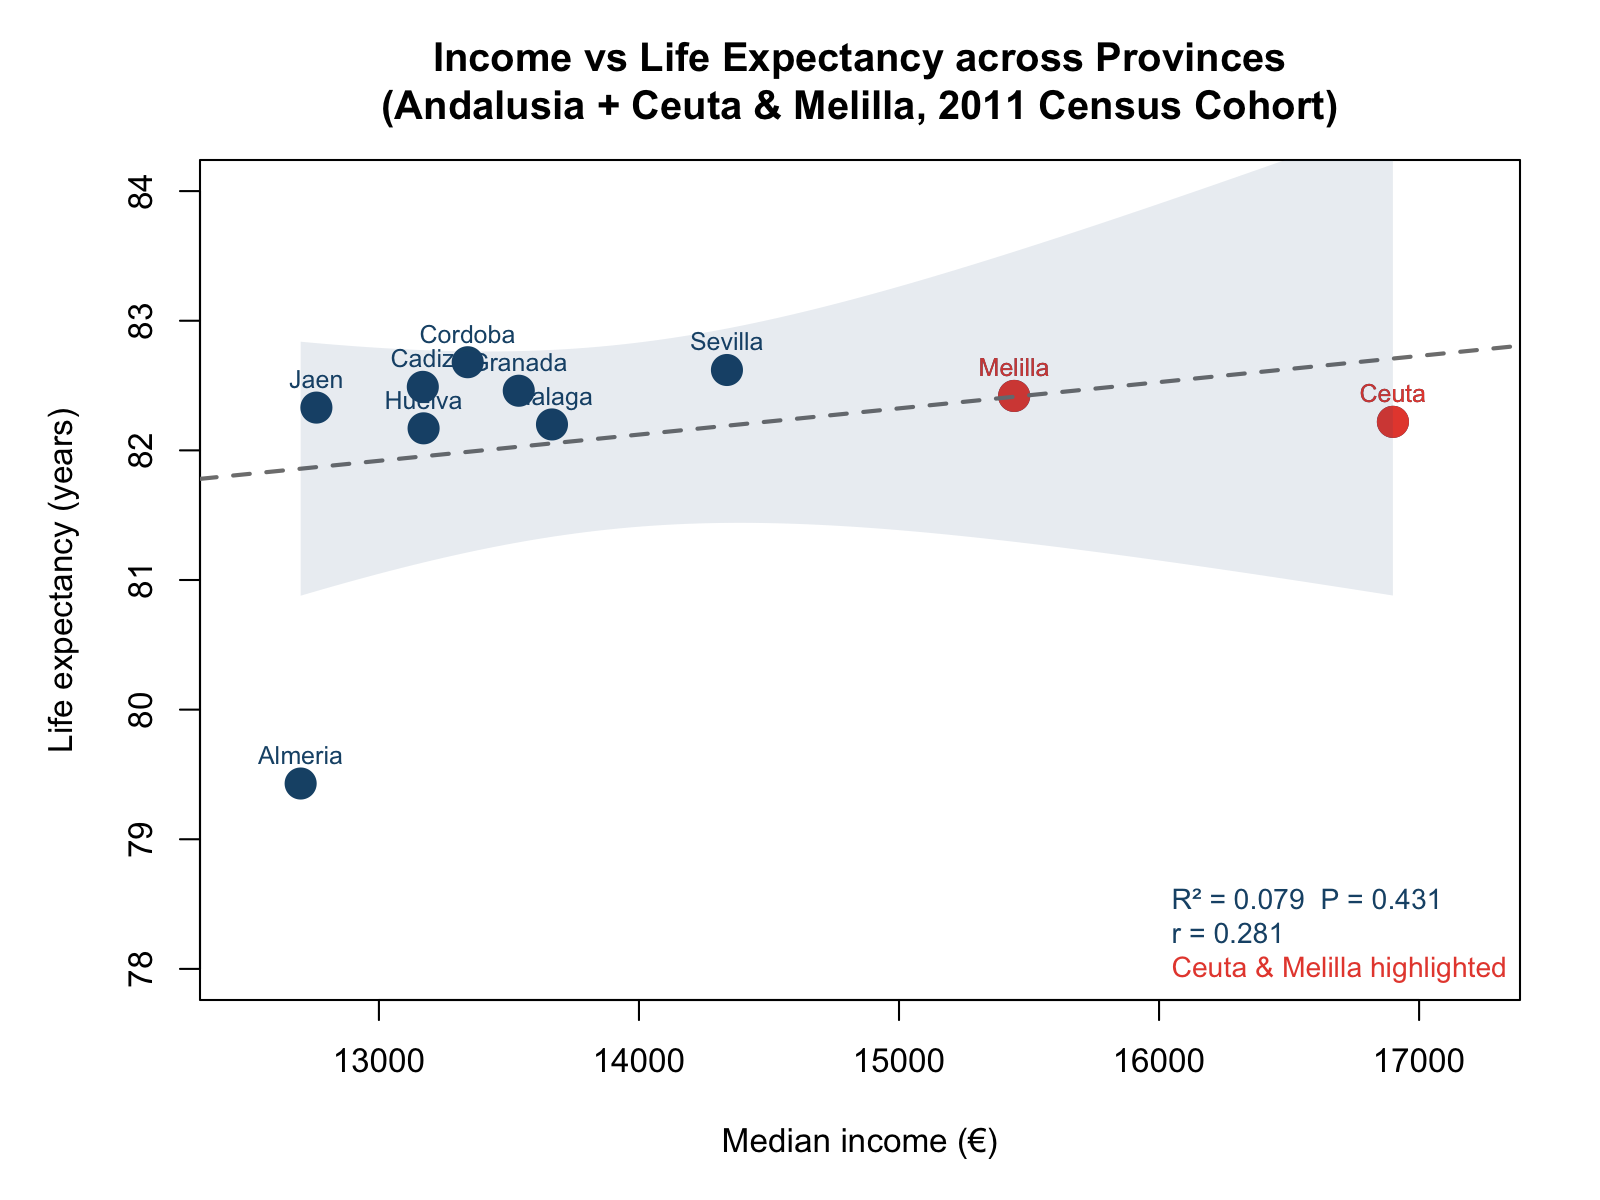
\includegraphics[keepaspectratio]{figures/renta_vs_ev_scatter.png}}

}

\caption{\label{fig-scatter}Scatter plot with loess smoother and linear
regression (R\^{}2 = 0.04, p = 0.62).}

\end{figure}%

\subsection{Interactive application}\label{interactive-application}

The RENTASALUD Shiny application integrates all findings across five
interactive tabs. The \emph{Explorar} tab features choropleth maps with
a year slider (2015--2022) for animating temporal changes across 12
indicators. The \emph{Asistente IA} tab enables natural-language queries
via large language models (Ollama, OpenAI or Gemini). The
\emph{Relaciones} tab presents scatter plots with loess smoothers,
cluster dendrograms and grouped bar charts of life expectancy by
province and sex. The \emph{Causas Mortalidad} tab provides interactive
cause-of-death decomposition with horizontal bar charts, searchable
tables and age-band life expectancy curves. The \emph{Metodología} tab
documents all indicator definitions. Source code:
\href{https://github.com/migariane/RENTASALUD}{github.com/migariane/RENTASALUD}.

\section{Discussion}\label{discussion}

\subsection{Principal findings}\label{principal-findings}

This study provides the first integrated, interactive atlas of income,
demography and life expectancy for Andalusia. Life expectancy at birth
(79.5 years for men, 84.4 for women) falls below the Spanish national
average (\textasciitilde80.5 and \textasciitilde86.0 years,
respectively) (Instituto Nacional de Estadística 2024), consistent with
Andalusia's historically lower socioeconomic indicators. The dominance
of malignant tumours and circulatory diseases as causes of premature
mortality---together accounting for approximately 7 years of potential
life expectancy gain in men and 6 in women---aligns with European
preventable mortality patterns (Beltrán-Sánchez et al. 2008; {Mackenbach
et al.} 2015) and reinforces the continued importance of cancer
screening, cardiovascular risk prevention and smoking cessation
interventions. The larger tumour impact in men (+1.1 years vs women)
reflects Spain's historically higher male smoking prevalence, a gap that
is narrowing in younger cohorts.

\subsection{Geographical scale and the income--longevity
gradient}\label{geographical-scale-and-the-incomelongevity-gradient}

The weak and non-significant provincial-level income--longevity
correlation (r = 0.21; 95\% CI: -0.59 to 0.81) contrasts sharply with
the steep census-tract gradients reported by Redondo-Sánchez et al.
(Redondo-Sánchez et al. 2022), who found a gap of 3.8 years for men and
3.2 years for women between the most and least deprived census tracts
nationally. This discrepancy, spanning an order of magnitude,
illustrates the modifiable areal unit problem (MAUP): provincial
aggregation masks substantial intra-provincial heterogeneity in both
income and mortality. The Southern European pattern of smaller health
inequalities ({Mackenbach et al.} 2018; Regidor et al. 2012) does not
imply absence of a socioeconomic gradient; rather, the gradient operates
at finer spatial scales and may be mediated by different
mechanisms---including dietary patterns, social networks and universal
healthcare---compared to Northern or Eastern Europe. These findings
imply that area-based interventions should target the most deprived
census sections, and RENTASALUD is designed precisely to facilitate this
through interactive sub-provincial mapping.

\subsection{Strengths and limitations}\label{strengths-and-limitations}

The main strength is the integration of individual-level longitudinal
mortality follow-up from the BDLPA (\textasciitilde637,000 individuals,
12 years) with granular census-section socioeconomic data within an
open-source, reproducible platform featuring an AI-powered query
interface. Several limitations should be acknowledged. First, life
expectancy was estimated only at the provincial level, the most
important limitation; future work should pursue BDLPA--Padrón Continuo
linkage to recover census-section codes for small-area Bayesian
estimation. Second, period life tables assume constant age-specific
mortality rates, which may not hold during periods of rapid change.
Third, sample sizes limit precision at extreme ages (0--4 and 90+) when
disaggregating by province and sex. Fourth, there is a partial temporal
mismatch between income data (2015--2022) and mortality follow-up
(2011--2023). Fifth, cause-deleted decomposition assumes independence
between causes, meaning gains from eliminating multiple causes are not
additive.

\section{What is already known on this
topic}\label{what-is-already-known-on-this-topic}

\begin{itemize}
\tightlist
\item
  Socioeconomic deprivation is strongly associated with mortality in
  Spain, with a gap of 3.2--3.8 years between most and least deprived
  census tracts.
\item
  Southern Europe exhibits smaller educational inequalities in mortality
  than Northern or Eastern Europe.
\item
  Interactive tools integrating income and life expectancy at fine
  geographical scales remain scarce.
\end{itemize}

\section{What this study adds}\label{what-this-study-adds}

\begin{itemize}
\tightlist
\item
  RENTASALUD provides the first open-source interactive atlas of
  census-section income and life expectancy for Andalusia.
\item
  Provincial-level income--longevity correlation is weak (r = 0.21), in
  contrast to steep census-tract gradients.
\item
  Malignant tumours and circulatory diseases account for
  \textasciitilde7 years of potential life expectancy gain in men.
\item
  An AI-powered natural language interface enables non-specialist
  querying of the data.
\end{itemize}

\section{Acknowledgements}\label{acknowledgements}

Supported by the Plan Propio de Investigación y Transferencia,
University of Granada (2025, Programa 21). BDLPA data provided by the
IECA.

\section{Data Availability}\label{data-availability}

Source code:
\href{https://github.com/migariane/RENTASALUD}{github.com/migariane/RENTASALUD}.
Shiny app: {[}shinyapps.io link{]}. BDLPA microdata available from IECA
on request.

\section*{References}\label{references}
\addcontentsline{toc}{section}{References}

\protect\phantomsection\label{refs}
\begin{CSLReferences}{1}{1}
\bibitem[\citeproctext]{ref-beltran-sanchez2008}
Beltrán-Sánchez, Hiram, Samuel H. Preston, and Vladimir Canudas-Romo.
2008. {``An Integrated Approach to Cause-of-Death Analysis:
Cause-Deleted Life Tables and Decompositions of Life Expectancy.''}
\emph{Demographic Research} 19: 1565--602.
\url{https://doi.org/10.4054/DemRes.2008.19.35}.

\bibitem[\citeproctext]{ref-chiang1968}
Chiang, Chin Long. 1968. \emph{Introduction to Stochastic Processes in
Biostatistics}. (New York).

\bibitem[\citeproctext]{ref-ine2024}
Instituto Nacional de Estadística. 2024. \emph{Indicadores de
Mortalidad: Esperanza de Vida Al Nacer}.
\url{https://www.ine.es/jaxiT3/Tabla.htm?t=1415}.

\bibitem[\citeproctext]{ref-mackenbach2015}
{Mackenbach, Johan P., Ivana Kulhánová, Gwenn Menvielle, et al.} 2015.
{``Trends in Inequalities in Premature Mortality: A Study of 3.2 Million
Deaths in 13 European Countries.''} \emph{Journal of Epidemiology and
Community Health} 69 (3): 207--17.
\url{https://doi.org/10.1136/jech-2014-204319}.

\bibitem[\citeproctext]{ref-mackenbach2018}
{Mackenbach, Johan P., José R. Valverde, Barbara Artnik, et al.} 2018.
{``Trends in Health Inequalities in 27 European Countries.''}
\emph{Proceedings of the National Academy of Sciences} 115 (25):
6440--45. \url{https://doi.org/10.1073/pnas.1800028115}.

\bibitem[\citeproctext]{ref-marmot2010}
Marmot, Michael. 2010. \emph{Fair Society, Healthy Lives: The Marmot
Review}. University College London.

\bibitem[\citeproctext]{ref-redondo2022}
Redondo-Sánchez, Daniel, Marı́a-José Sánchez, Pablo Fernández-Navarro,
Bernard Rachet, and Miguel Angel Luque-Fernandez. 2022. {``Association
of Socioeconomic Deprivation with Life Expectancy and All-Cause
Mortality in Spain, 2011-2013.''} \emph{Scientific Reports} 12 (1):
15554. \url{https://doi.org/10.1038/s41598-022-19859-1}.

\bibitem[\citeproctext]{ref-regidor2012}
Regidor, Enrique, Anton E. Kunst, Fernando Rodríguez-Artalejo, and Johan
P. Mackenbach. 2012. {``Small Socio-Economic Differences in Mortality in
Spanish Older People.''} \emph{European Journal of Public Health} 22
(1): 80--85. \url{https://doi.org/10.1093/eurpub/ckr051}.

\bibitem[\citeproctext]{ref-regidor2014}
{Regidor, Enrique, Laura Reques, María José Belza, et al.} 2014.
{``Education and Mortality in Spain: A Review of the Literature.''}
\emph{Gaceta Sanitaria} 28 (6): 492--98.
\url{https://doi.org/10.1016/j.gaceta.2014.06.001}.

\end{CSLReferences}




\end{document}
